\documentclass{standalone}
\usepackage{tikz}
\usetikzlibrary{arrows.meta, bending}

\begin{document}

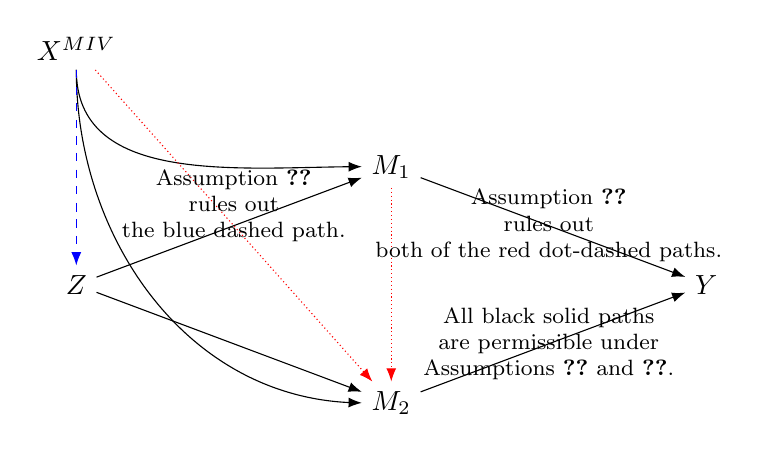
\begin{tikzpicture}[>=Latex, node distance=2cm]

% Define the positions of the nodes
\node (X_MIV) at (0,3) {$X^{MIV}$};
\node (Z) at (0,0) {$Z$};
\node (M1) at (4,1.5) {$M_1$};
\node (M2) at (4,-1.5) {$M_2$};
\node (Y) at (8,0) {$Y$};

% Draw black solid arrows
\draw[->] (X_MIV) to[out=-90,in=180] (M1);
\draw[->] (X_MIV) to[out=-90,in=180] (M2);
\draw[->] (Z) -- (M1);
\draw[->] (Z) -- (M2);
\draw[->] (M1) -- (Y);
\draw[->] (M2) -- (Y);

% Draw blue dashed arrow
\draw[blue, dashed, ->] (X_MIV) to[out=-90,in=90] (Z);

% Draw red dot-dashed arrows
\draw[red, densely dotted, ->] (M1) -- (M2);
\draw[red, densely dotted, ->] (X_MIV) -- (M2);

% Add labels for assumptions
\node[align=center, font=\footnotesize] at (2,1) {Assumption \ref{cond:irre1}\\rules out\\the blue dashed path.};
\node[align=center, font=\footnotesize] at (6,0.75) {Assumption \ref{cond:irre2}\\rules out\\both of the red dot-dashed paths.};
\node[align=center, font=\footnotesize] at (6,-0.75) {All black solid paths\\are permissible under\\Assumptions \ref{cond:irre1} and \ref{cond:irre2}.};

\end{tikzpicture}

\end{document}